\documentclass[tikz, border=10pt]{standalone}

\usepackage{tikz}
\usepackage{amsmath, amsfonts, amssymb, mathtools}

\begin{document}
    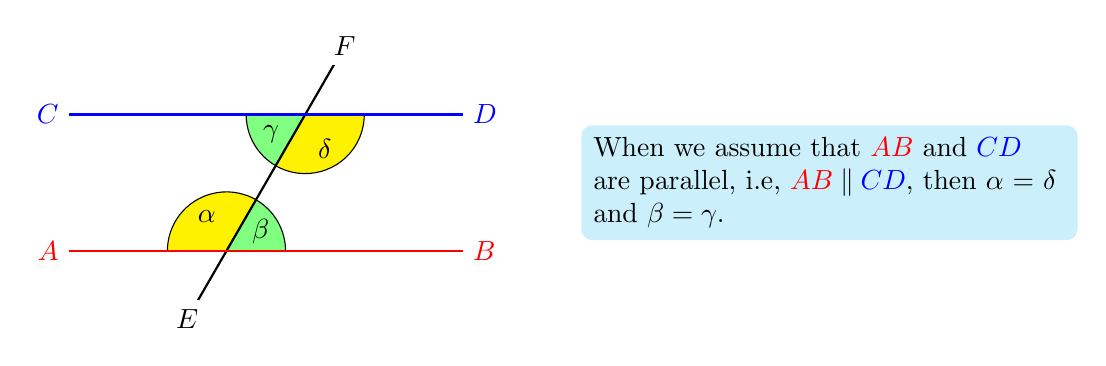
\begin{tikzpicture}
        \draw[fill=yellow] (0, 0) -- (60:0.75cm) arc (60:180:0.75cm);
        \draw (120:0.5cm) node {$\alpha$};
        \draw[fill=green!50] (0, 0) -- (right:0.75cm) arc (0:60:0.75cm);
        \draw (30:0.5cm) node {$\beta$};
        
        \begin{scope}[shift={(60:2cm)}]
            \draw[fill=green!50] (0, 0) -- (180:0.75cm) arc (180:240:0.75cm);
            \draw (210:0.5cm) node {$\gamma$};
            \draw [fill=yellow] (0, 0) -- (240:0.75cm) arc (240:360:0.75cm);
            \draw (-60:0.5cm) node {$\delta$};
        \end{scope}
        
        \begin{scope}[thick]
            \draw (60:-1cm) node[fill=white] {$E$} -- (60:3cm) node[fill=white] {$F$};
            \draw[red] (-2, 0) node[left] {$A$} -- (3, 0) node[right] {$B$};
            \draw[blue, shift={(60:2cm)}] (-3, 0) node[left] {$C$} -- (2, 0) node[right] {$D$};
        \end{scope}
        
        \draw[shift={(60:1cm)}, xshift=4cm] 
            node[right, text width=6 cm, rounded corners, fill=cyan!20, inner sep=1ex]{
                When we assume that \textcolor{red}{$AB$} and \textcolor{blue}{$CD$} are parallel, i.e, $\textcolor{red}{AB}\mathbin{\|}\textcolor{blue}{CD}$, then $\alpha=\delta$ and $\beta=\gamma$.
            };
    \end{tikzpicture}
\end{document}